\documentclass[11pt,a4paper, final, twoside]{article}
%%%%%%%%%%%%%%%%%%%%%%%%%%%%%%%%%%%%%%%%%%%%%%%%%%%%%%%%%%%%%%%%%%%%%%%%%%%%%%%%%%%%%%%%%%%%%%%%%%%%%%%%%%%%%%%%%%%%%%%%%%%%%%%%%%%%%%%%%%%%%%%%%%%%%%%%%%%%%%%%%%%%%%%%%%%%%%%%%%%%%%%%%%%%%%%%%%%%%%%%%%%%%%%%%%%%%%%%%%%%%%%%%%%%%%%%%%%%%%%%%%%%%%%%%%%%
\usepackage{amsmath}
\usepackage{fancyhdr}
\usepackage{amsthm}
\usepackage{amsfonts}
\usepackage{amssymb}
\usepackage{amscd}
\usepackage{latexsym}
\usepackage{graphicx}
\usepackage{graphics}
\usepackage{natbib}
\usepackage[colorlinks=true, urlcolor=blue,  linkcolor=black, citecolor=black]{hyperref}
\usepackage{color}
\usepackage{natbib}
\usepackage{sectsty}
\usepackage{subcaption}
\usepackage{caption}
\usepackage{indentfirst}
\setcounter{MaxMatrixCols}{10}



\sectionfont{\fontsize{12}{15}\selectfont}

\renewcommand{\thefootnote}{}
\setlength{\oddsidemargin}{1pt} \setlength{\evensidemargin}{1pt}
\setlength{\hoffset}{-1in} \addtolength{\hoffset}{25mm}
\setlength{\textwidth}{140mm} 
\setlength{\marginparsep}{0pt} \setlength{\marginparwidth}{0pt}
\setlength{\topmargin}{0pt}
\setlength{\voffset}{-2in} \addtolength{\voffset}{20mm}
\setlength{\textheight}{260mm}
\setlength{\headsep}{20mm}
\setlength{\footskip}{15mm}
\pagestyle{fancy}
\fancyhead{} \fancyfoot{} 



%       Theorem environments
\newtheorem{thm}{Theorem}[section]
\newtheorem{algorithm}[thm]{Algorithm}
\newtheorem{axiom}[thm]{Axiom}
\newtheorem{lem}[thm]{Lemma}
\newtheorem{example}[thm]{Example}
\newtheorem{exercise}[thm]{Exercise}
\newtheorem{notation}[thm]{Notation}
\newtheorem{problem}[thm]{Problem}
\theoremstyle{proposition}
\newtheorem{prop}{Proposition}[section]
\newtheorem{case}[thm]{Case}
\newtheorem{claim}[thm]{Claim}
\newtheorem{conclusion}[thm]{Conclusion}
\newtheorem{condition}[thm]{Condition}
\newtheorem{conjecture}[thm]{Conjecture}
\newtheorem{cor}[thm]{Corollary}
\newtheorem{criterion}[thm]{Criterion}
\theoremstyle{definition}
\newtheorem{defn}{Definition}[section]
\theoremstyle{remark}
\newtheorem{rem}{Remark}[section]
\newtheorem{solution}[thm]{Solution}
\newtheorem{summary}[thm]{Summary}
\numberwithin{equation}{section}
\renewcommand{\rmdefault}{phv} % Arial
\renewcommand{\sfdefault}{phv} % Arial
\pagenumbering{arabic} % 1, 2, 3, 4, ...

\input{macros}


\begin{document}
\hyphenpenalty=100000


\sloppypar

\begin{center}

{\Large \textbf{\\User Customization of Caregiving Robots that \\Support Older Adults with Dementia}}\\[5mm]
{\large \textbf{Zehui (Joyce) Zhou}\\[1mm]}
{\normalsize \emph{Under the supervision of Professor Sheila McIlraith,\\ Dr.\ Steven Shapiro, and Dr.\ Richard Valenzano}\\[1mm]}
\end{center}


\section{Introduction}\label{I1}
Dementia affects more than 35 million people worldwide, and the number is still growing dramatically. Dementia affects people's ability to live independently, thus many dementia patients face the prospect of being institutionalized. As home care is often costly, we are investigating the development of an affordable socially assistive robot to support cognitively impaired older adults with daily living activities, which will potentially extend their time living at home.

To communicate with patients effectively, a caregiving robot should tailor its interactions to its interlocutors, taking into account the nature and degree of cognitive impairment, other health issues, and individual preferences.
\section{Approach}\label{I2}
We equipped the robot with a knowledge base embodying ``best practices'' for communicating with different classes of individuals \cite{practice1,practice2, rochon, web1, web2, web3}. Upon delivery, the knowledge base can be augmented with (some) information about the people with whom the robot is expected to interact. When communicating with an individual, the robot uses the knowledge base to determine a customized strategy.

People with dementia often have difficulty completing daily tasks.
In this work, we customized the interactions of the robot with users of the COACH system, which provides assistance to complete the task of handwashing~\cite{COACH}.
COACH tracks the user's hand positions to ensure that he or she is following a proper sequence to wash their hands.  
If COACH determines that the user is having difficulty, it will provide audio or video instructions, called \emph{prompts}. These prompts are then customized by our system.

\section{Implementation}\label{I3}
COACH uses a POMDP-based \emph{Task Manager} to estimate the user's progress and determine the next prompt.
The prompt is then processed by the \emph{Executor} which plays a pre-recorded audio or video clip
(see Fig.~\ref{fig:COACH}).

To customize the behaviour of COACH, we deployed a \emph{Prompter} which reasons using features stored in the knowledge base to adapt the prompt for the user. 
We also modified the Executor so that it could use the output of the Prompter to dynamically generate an appropriate audio clip, rather than simply using a pre-recorded one (see Fig.~\ref{fig:COACH_with_customization}).
\begin{figure}[h!]
        \centering
        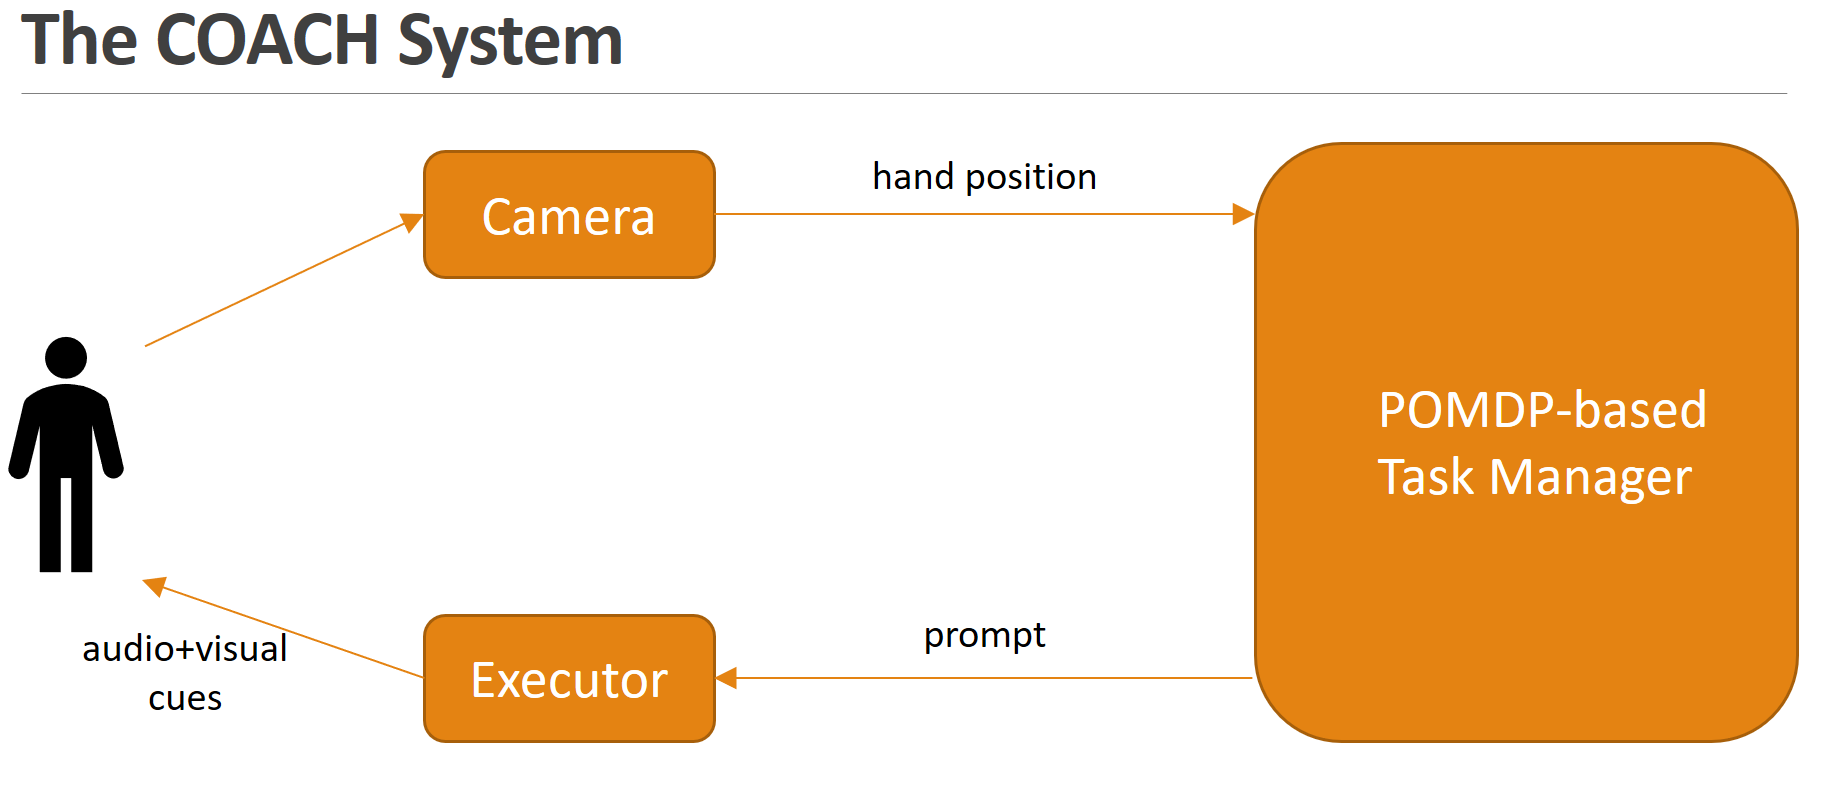
\includegraphics[width=0.8\textwidth]{COACH_prompt.png}
        \caption{The original COACH system.}
        \label{fig:COACH}
\end{figure}
\begin{figure}[h!]
        \centering
        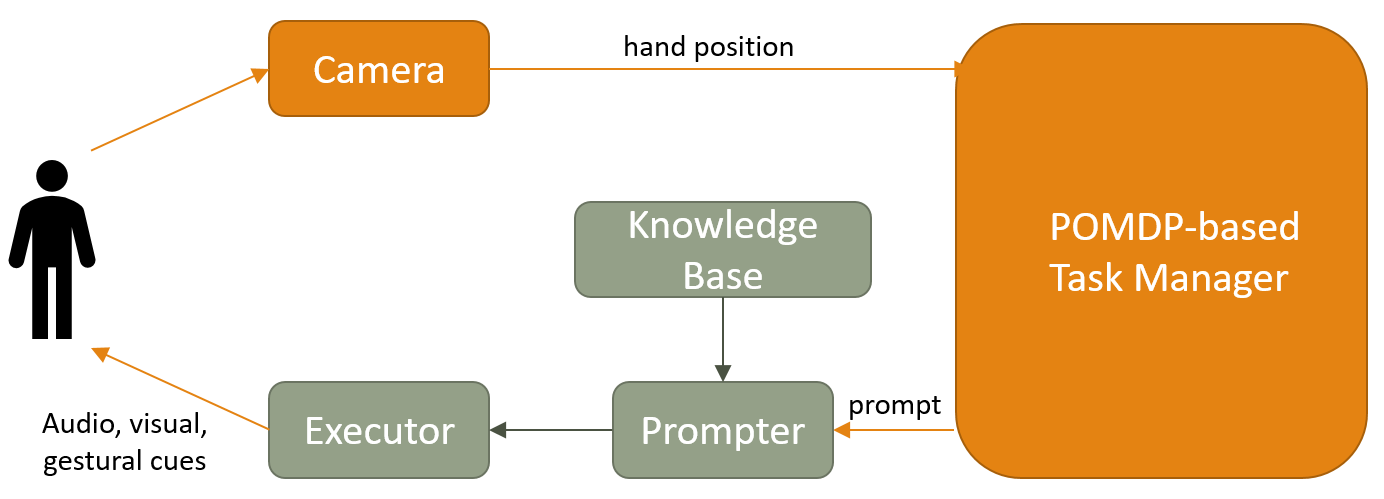
\includegraphics[width=0.8\textwidth]{COACH_with_customization_prompt.png}
        \caption{COACH system with customization.}
        \label{fig:COACH_with_customization}
\end{figure}
\par
%\noindent The \textbf{Prompter} is the module deciding how should a customized prompt be carried out.\\ % duplicates earlier info
\emph{Universal parameters} --- such as prompt detail level, volume, voice type, and speed --- are determined using  the knowledge base.
Using these parameters, the prompt from the Task Manager, and other relevant information (e.g., how the user likes to be addressed, what kind of soap is in the environment), the Prompter generates a customized prompt and mode of delivery. This allows for different types of prompts for different users and situations.
%The \textbf{Executor} is responsible for content display and voice generation. IBM's \textbf{Watson} is then used to synthesize the audio clip. 
The Executor then uses IBM's Watson to synthesize the audio clip (see Fig.~\ref{fig:arch}). 
\begin{figure}[h!]
    \centering
    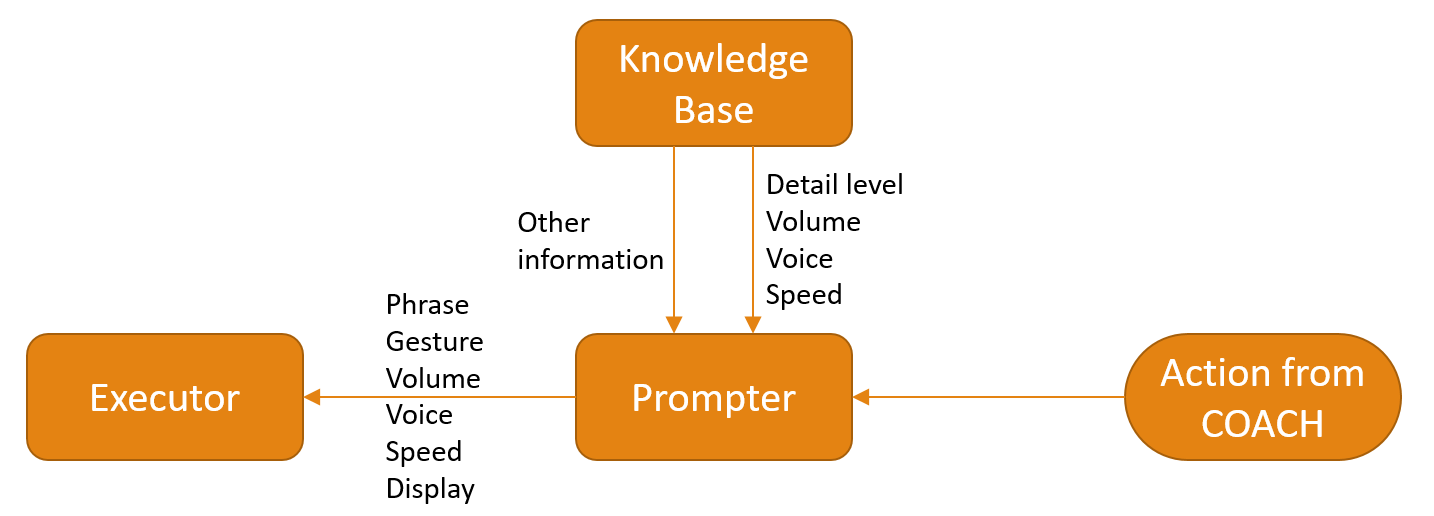
\includegraphics[width=0.8\textwidth]{prompter.png}
    \caption{The architecture of the Prompter.}
    \label{fig:arch}
\end{figure}\\

\section{Illustrative Examples}\label{I4}
The original COACH system does not take the user and the environment into consideration.
Consider the following example prompt, in which the Task Manager decides the user should turn on the tap.
\begin{center}
{\color{red} Original COACH Pre-recorded Prompt}
\end{center}
\begin{center}
\textbf{\textit{``Try pulling the silver lever towards you."}}
\end{center}
\noindent Now, we show three examples of prompts that our system generates instead, depending on individual circumstances. Note that both the content and mode of delivery vary according to the individual.
\begin{center}
    {\color{red}Customized Prompts Based on Context}
\end{center}

{\bf Scenario 1:} The user is an elderly woman that has severe dementia and hearing difficulty.
\begin{center}
\textbf{\textit{``Ms.\ Marth, now turn on the tap.''}}
\end{center}
%\begin{flushright}
The user is addressed formally (as desired) using a short sentence.  This prompt is generated using a
low-pitched voice, high volume, and slow speed.\\
%\end{flushright}
%She was addressed formally (as desired) using a short sentence.\\

{\bf Scenario 2:} The user is an elderly Spanish-speaking woman with mild dementia and mild hearing difficulty.
\begin{center}
\textbf{\textit{``Se\~nora Abar, saque un poco de agua.''}}
\end{center}
%
The user is addressed formally in Spanish (as desired)
using a short sentence.  This prompt is generated using normal volume and normal speed.\\

{\bf Scenario 3:} The user is a 4 year-old girl.
\begin{center}
\textbf{\textit{``Vivian, now turn on the tap. Be careful with the hot water.''}}
\end{center}
%\begin{flushright}
The user is addressed by first name using multiple sentences,
with a high-pitched voice, normal volume, and normal speed.
%\end{flushright}
Being a child, she was also reminded of potential danger.

%In all the cases, we believe the customized prompt is better suited for the situation at hand.

\section{Evaluation}
To evaluate the effectiveness of the customizations, we propose using the following criteria.

\emph{Effectiveness}: Effectiveness measures how successful our approach is at helping users complete the handwashing task? We plan to evaluate this in trials by measuring the success rate of completing the task, and the number of prompts used per session.

\emph{Satisfaction}: Satisfaction measures how satisfied users feel with the help provided by the robot. We would use a questionnaire completed by the user(s) and/or expert observers to provide feedback on individual satisfaction with the robot's behaviour.

These kinds of evaluations require human trials. Due to the need for ethics approval, the evaluation is left for future work.

\section{Conclusion}
We customized the daily task of handwashing to demonstrate how human-robot interaction can be tailored using a knowledge base embodying best practices, taking into account individual circumstances and preferences. Our customizations adapt the robot's interactions to the nature and degree of cognitive impairment, other health issues, as well as personal preferences, such as language choice. 

%Due to the scope of hand-washing task, the customization is limited. The customization we implemented failed to show the potential of tailor its behaviour with respect to user's preference.

\section{Future Work}
% work shows the potential and limitation of customization of handwashing task using knowledge base. There are some works should be done in the future.
We plan to explore the use of Reinforcement Learning to adapt customizations through interaction with the user. Since people's preferences and impairments can change over time, and the initial knowledge base may require some tuning, the robot should be able to learn about its users and incorporate the new knowledge into its interactions.

As our goal is to create a socially assistive robot to support cognitively impaired older adults with daily living activities, the robot may need to help with different kinds of activities, such as tea or meal preparation.
The system can also be expanded to use other languages than English or Spanish.
Finally, our customization techniques should undergo evaluation. We have discussed some strategies for evaluation above, however we will investigate other strategies as well, and evaluate the system.\\


\noindent \textbf{Acknowledgements}\\

\noindent We would like to thank our collaborators: CrossWing Inc.; Professor Alex Mihailidis and team at the Toronto Rehabilitation Institute; Professor Goldie Nejat and team in Mechanical and Industrial Engineering at the University of Toronto; and Professor Fran\c{c}ois Michaud and team at the University of Sherbrooke.  We also wish to thank Dr.~Elizabeth Rochon from the Toronto Rehabilitation Institute for her expert advice on suitable strategies for communicating with persons with dementia.
Computations were performed on the SOSCIP Consortium's Cloud Data Analytics computing platform. SOSCIP is funded by the Federal Economic Development Agency of Southern Ontario, the Province of Ontario, IBM Canada Ltd., Ontario Centres of Excellence, Mitacs and 15 Ontario academic member institutions.


\bibliography{extended_abstract}
\bibliographystyle{unsrt}

\end{document}

